\documentclass[a4paper]{article}
\usepackage[T1]{fontenc}
\usepackage[utf8]{inputenc}
\usepackage{lmodern}
\usepackage{graphicx}
\usepackage{hyperref}
%\usepackage{tipa}

\usepackage{setspace} 
\DeclareUnicodeCharacter{00A0}{ }

\begin{document}
\begin{titlepage}

\newcommand{\HRule}{\rule{\linewidth}{0.7mm}} % Defines a new command for the horizontal lines, change thickness here


\center % Center everything on the page
 
%----------------------------------------------------------------------------------------
%	HEADING SECTIONS
%----------------------------------------------------------------------------------------

\textsc{\LARGE University of Tromsø}\\[1.5cm] % Name of your university/college
\textsc{\Large INF-2900}\\[0.5cm] % Major heading such as course name
\textsc{\large Software Engineering}\\[0.5cm] % Minor heading such as course title

%----------------------------------------------------------------------------------------
%	TITLE SECTION
%----------------------------------------------------------------------------------------

\HRule \\[0.5cm]
{ \huge \bfseries Turi}\\[0.5cm] % Title of your document
\HRule \\[3cm]
 
%----------------------------------------------------------------------------------------
%	AUTHOR SECTION
%----------------------------------------------------------------------------------------

% If you don't want a supervisor, uncomment the two lines below and remove the section above
\Large \emph{Group:}\\
1\\[2cm] % Your name
% title
%----------------------------------------------------------------------------------------
%	DATE SECTION
%----------------------------------------------------------------------------------------

\textsc{\large Spring 2015}\\[4cm] % Date, change the \today to a set date if you want to be precise

%----------------------------------------------------------------------------------------
%	LOGO SECTION
%----------------------------------------------------------------------------------------


\includegraphics{pictures/UiT_samarbeidslogo_bokmal_300ppi.png}\\[1cm] 
% Include a department/university logo - this will require the graphicx package
 
%----------------------------------------------------------------------------------------

\vfill % Fill the rest of the page with whitespace

\end{titlepage}
% END TITLE PAGE %

\tableofcontents
\pagebreak


\section{Introduction}
Imagine you want to go on a trip - to Norway for example. You ask you friends to join you but they reject because they can not afford the money or they have no spare time. What now? You can either go alone or try to find some people who can join you. The first place we look today is on the world wide web. We already can find some portals where you can find partners for your trip. But what about planning your actually trip? We couldn’t find a tool which allows you to plan your trip in detail. Planning your trip gets especially difficult if you find your trip mates online and you can not meet because you live too far away from each other. You can now either use the phone or create e.g. some Facebook group. Still those ways lack of several features we want to implement in our trip planner which makes it unique. In fact we came up with the idea to create a a trip planner which offers a combination between socialising and planning for your trips.

\subsection{The product name: turi}
The name derived from the Norwegian word “tur” (a trip/a walk). turi was short and pregnant enough and sounds best to the ear. It is also a Norwegian name, but this will be no problem when we think about topics like a trademark etc.

\subsection{Summary of goals (planned functionalities)}
The following functionalities should be supported (bold means that we they were implemented during the course sprints):
\begin{itemize}
  \item {\textbf{Discuss with participants}}
  \item {\textbf{Event management (for appointments top plan)}}
  \item {\textbf{Route planning}}
  \item {\textbf{Equipment planning}}
  \item {\textbf{Gallery to visualize your trip experiences}}
  \item {\textbf{Blog about your experience}}
  \item {\textbf{Share your trip (public/private)}}
  \item {Copy a previous trip from others (e.g. routes)}
  \item {Rating functionality and other common social functions (commenting, likes..)
  \begin{itemize}
    \item {Friend requests}
  \end{itemize}}
  \item {\textbf{Explore trips based on their location}}
  \item {Badges and rewards for participating and using Turi}
  \item {Search and find trips according your interests}
\end{itemize}

\noindent
Finally we were not able to implement all of our goals and we had tons of more ideas. But for the first release of turi (1.0.0) we decided to require all these features above.


\section{The development process}
\subsection{Git}
We use github.com instead of the git repository supplied to us from the school, this gave us the opportunity to work outside the school network. In addition it gave us the ability to use 3rd party applications, this is explained the following subsections. The githib repository address is: https://github.com/turi-inc/turi.

\subsubsection{Travis CI}
Travis CI is a hosted continuous integration service. It is integrated with GitHub and provides testing for our project. So when we created a pull request on the development branch of the Github repository, Travis would test our new code automatically and give us a clear indication if the test was passing or not. When the pull request is merged with the development branch it would be tested once again by Travis to be sure that everything was working correctly before the pull request is automatically merged with the master branch of the repository. The log from Travis is public and can be seen here: https://travis-ci.org/turi-inc/turi/builds.

\begin{figure}
  \begin{center}
    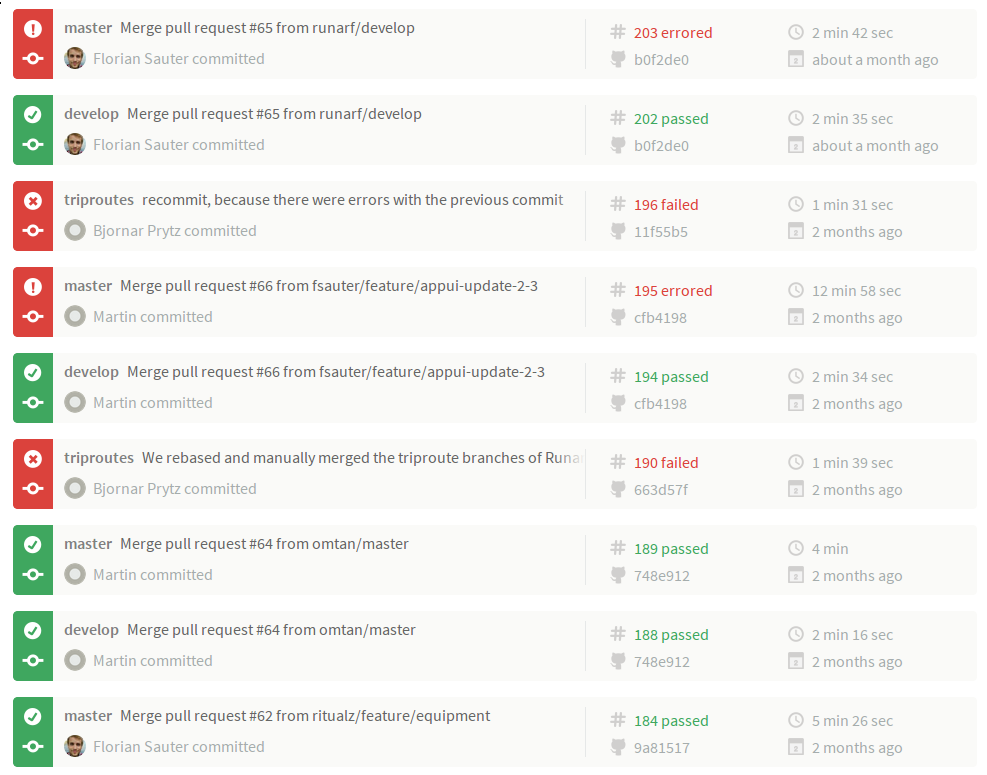
\includegraphics[scale=0.45]{pictures/Travis_buildlog.png}
    \caption{A sample of the build logs from Travis CI}
    \label{fig:}
  \end{center}
\end{figure}


\subsubsection{Heroku}
Heroku is a cloud platform which host our project for free. When a pull request is merged with the master branch it's automatically pushed to Heroku. This gives us and other people to see a preview of the project. We had some minor problem getting this to work properly since we use Sqlite3 when we develop, but Heroku does not support this and so we had to switch over to postgres in the production environment.

\subsubsection{CodeClimate}
Is also a 3rd party application which checks our code for test coverage, complexity and duplications. The check is done on the master branch of the repository, every time a new pull request is merged with the branch. It gives us an indication about the code health and grades our code, on the basis of test coverage, complexity and duplications. The summary of the code climate of out project can be found here: https://codeclimate.com/github/turi-inc/turi. \\
CodeClimate also have some cool features like Trends over the "health" of our code over time, and the location "hotspots" in the code.  

\begin{figure}
  \begin{center}
    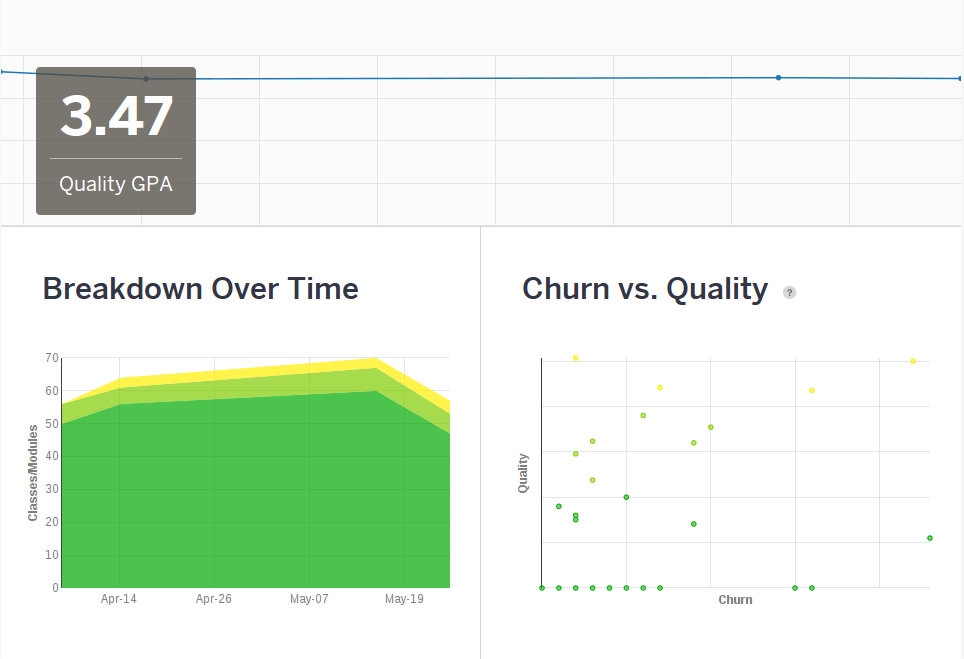
\includegraphics[scale=0.45]{pictures/trends_code.png}
    \caption{CodeClimate trends}
    \label{fig:}
  \end{center}
\end{figure}

\subsubsection{Hakiri}
This 3rd party application is used to show if there is any gem which is not up to date, and if there is any known security claws in any of the gems we use in our project.

\section{Design of the site}

\section{Gems}
We use several gems in our project, this means that we not need find up the wheel for already created features, and we can focus on our own feature. All the gems used can be found in the gemfile in the project source, but the most important ones are:
\subsection{Devise}
In the first iterations we created our own authentication system, but we found fast out that we could use \textit{Devise}. This made it possible to focus on other tasks and let \textit{Devise} handle the authentication. 

\subsection{Pundit}

\subsection{Leaflet}

\subsection{rails-asserts}

\subsection{Geocoder}
Geocoder is a so called "complete geocoding solution for Ruby"\cite{geocoder}, it provides a location based on IP, location and so on, in the project we use it for location based search, for example in the trip start and end location. 

\subsection{Puma}
Puma is a "simple, fast, threaded, and highly concurrent HTTP 1.1 server for Ruby/Rack applications."\cite{puma}. Heroku recommend Puma over the stock rails server (WEBrick) by saying that: "While WEBrick should be fine for development, it was not designed to handle a high concurrent workload that a Ruby app must serve in production. A production web server should be used instead."\cite{heroku_webserver}. Even tho Heroku only uses one core (for the free program), this secures that the project is ready for a deployment onto a multi-core server in the future.  


\section{Trip Features}
The trip and it's features are the main focus of our project. 
\subsection{Discuss}
\subsection{Event management}
\subsection{Equipment planning}
\subsection{Gallery}
\subsection{Blog}
\subsection{Share your trip (public setting)}
\subsection{Explore trips}
\subsection{Search}

\section{Other features}
\subsection{Friend requests}

\section{Tests}

\section{Group collaboration}


\section{The development process}

Using tools like GitHub and Travis CI we came up with the following workflow:

\subsection{Git Workflow}
Since we use Git together with GitHub, we are able to make use of the continuous integration tool Travis CI. Therefore we decided to go with the following development workflow. Please note that the term "origin" represents for the main turi repository on GitHub.


\subsubsection{Developing of a new feature}
The developer creates a local feature branch with a telling name. A feature always relates to a user story in Agilefant.


\subsubsection{Starting a merge request}
If the developer finished with the development of his local feature, he pushes the feature branch to his own remote repository (which is a fork of the origin repository). Before he pushes his changes, he has to do a rebase on the current develop branch of the origin to make sure all sources are up to date and we don't mess up the git history we thousand of branches. After making sure that everything is up to date, he can create a merge request on GitHub from his feature branch to the origin develop branch.

\subsubsection{Validating the merge request}
After the merge request is submitted, it's open for discussion. For additional validation, Travis builds every merge request to ensure that all tests are running. If the Travis CI build is passing and the merge request can be fast forwarded (so the request was rebased) another developer can accept the merge. The person who accepts the merge should be never be the owner of the merge request.

\subsubsection{Deploying to production}
A soon as a merge request is accepted, Travis CI will run again against the latest sources of the origin develop branch. If the build is successfull Travis will push the develop branch to the master branch. Therefore we will always have a stable version of turi on the master branch. A developer should never push changes directly to the master branch.

After a push to the master Travis will push the code to Heroku and run the database migrations. Therefore we always have a stable snapshot version on heroku.

\subsection{Conclusion of the workflow}


\end{document}

%puma
https://github.com/puma/puma

% heroku_webserver
https://devcenter.heroku.com/articles/ruby-default-web-server
